\subsection{Overview}
The following diagram represents the high level architecture of the system, including the external entities that will interact with it.
\\
\begin{figure}[H]
    \centering
    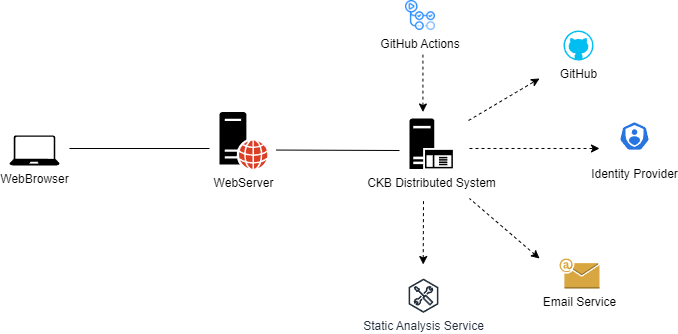
\includegraphics[width=1\textwidth]{Diagrams/overview.png}
    \caption{CKB system diagram}
    \label{overview_diagram}
\end{figure}
The main elements contained in Figure \ref{overview_diagram} are:
\begin{itemize}
    \item \textbf{WebBrowser}: used by students and educators to access the system functionalities through the web application.
    \item \textbf{WebServer}: the web server that hosts the web application of the system. Its role is storing, processing, delivering webpages to users and serving their requests.
    \item \textbf{CKB Distributed System}: the distributed system composed of multiple microservices that implement the core functionalities of the system. Its in charge of the data management, application and integration logic of the whole CKB platform.
    \item \textbf{External Entities}: the CKB Distributed System must be able to integrate with external actors to accomplish its functionalities. The arrow in the diagram highlights the direction of the interaction between the system and the external entities.
\end{itemize}
\subsection{Component view}
The following component diagram highlights the main components of the system and their interaction with external entities and services. In the diagram, the components have 
been organized to highlight the logical grouping of the system elements.\\The WebApplication component represents the presentation layer of the system, being the only entry point for the users.
The application and integration logic are represented together due to their tight interaction, while the data layer contains the databases accessed by the respective microservices.
Different colors are used to highlight components that share similar roles in the system.\\ \textcolor{orange}{Orange} components represent the system's microservices. Some complex microservices have been further decomposed into subcomponents, for a more fine grained representation.\\
\textcolor{yellow}{Yellow} components represent the model of the database accessed by its microservice. The model offers to the microservice an abstraction of the database, allowing it to access the data without knowing the underlying database implementation technology.\\ 
The \textcolor{violet}{violet} has been used to highlight components that cover an important role in the integration between some of the main microservices of the system. Specifically, it has been used for the queues subcomponents, which are used to implement the asynchronous and concurrent communication between specific microservices.
Some microservices have an important role in the integration with external entities as well, but have been depicted with their orange color used for microservices. This aspect will be clarified in the detailed description of the components that follows the diagram.\\
\textcolor{red}{Red} components represent the external services that interact with the system.\\
Finally, the \textcolor{green}{green} color has been used to highlight the databases components that are used to store the data of the system.\\
It's important to notice that for the sake of simplicity and readability, the interface offered by the ServiceRegistry has been depicted with some dotted arrows that connect all the microservices to it.
\begin{figure}[H]
    \centering
    \vspace{-3cm}
    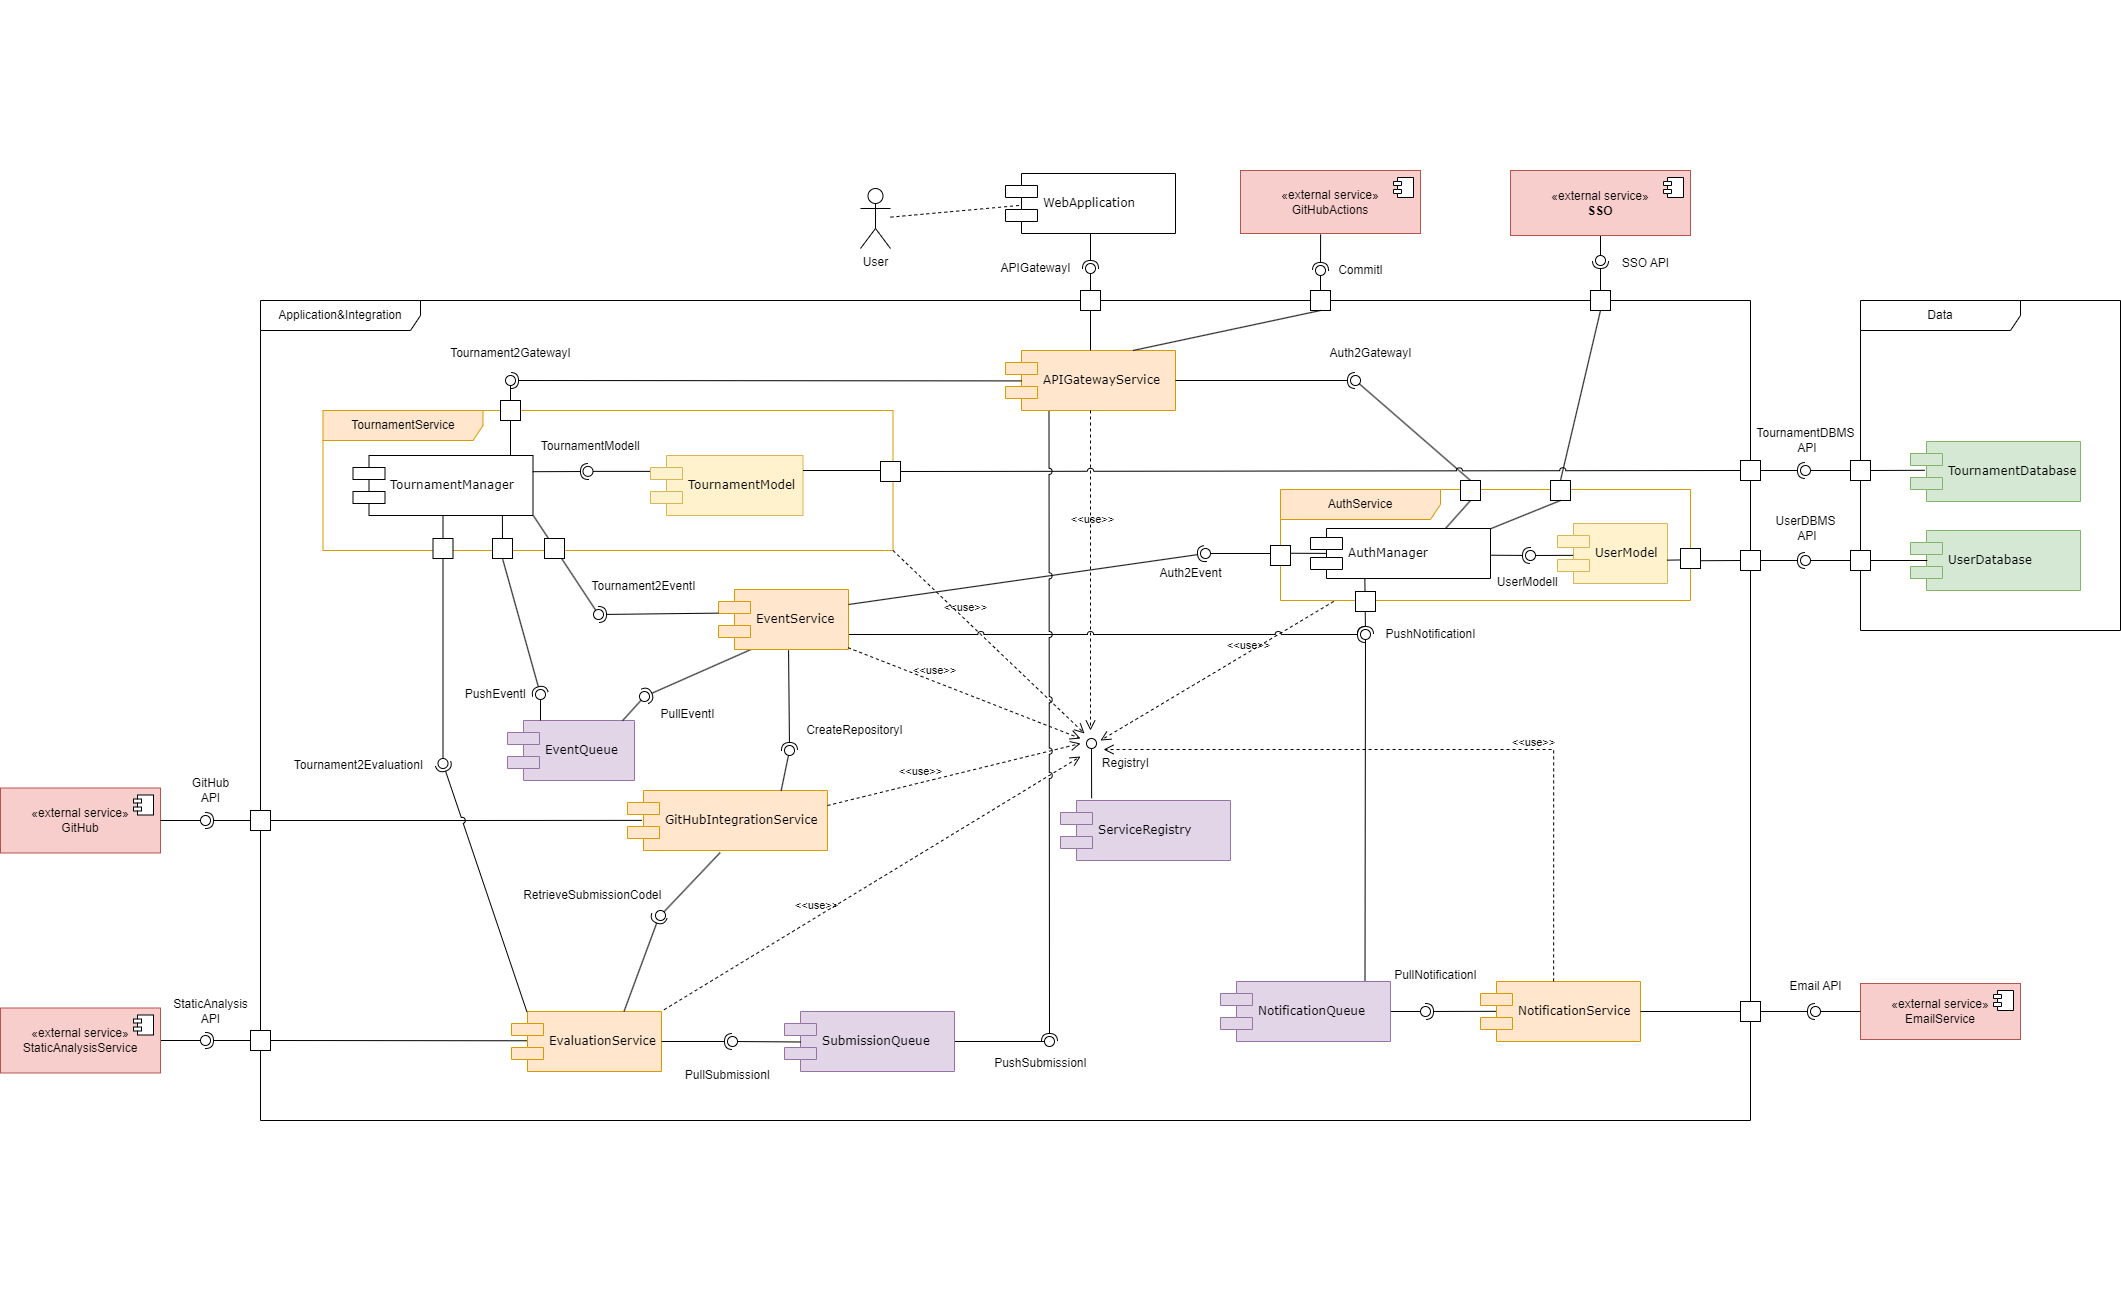
\includegraphics[width=1.6\textwidth,angle=90,origin=c]{Diagrams/component_diagram.png}
    \caption{Component diagram}
    \label{component_diagram}
\end{figure}
The components in Figure \ref{component_diagram} are :
\begin{itemize}
    \item \textbf{WebApplication}: the web app to which users of the CKB platform (students and educators) connect through a modern web browser. It is the front end of the system, and thanks to the interface offered by the \textbf{APIGatewayService}, allows users to manage and access the most important aspects of tournaments and battles
    \item \textbf{APIGatewayService}: this component is the microservice that exposes the REST API used by the WebApplication. Indeed, it allows the implementation of the main functionalities needed by the users of the web application. It also offers a REST API, used by the GitHub Actions Service, to notify a submission of a student on the Github repository.
    It's responsible for the following functionalities:
    \begin{itemize}
        \item Request validation and access limit: it is responsible for the validation of the requests, limiting the access to the system's APIs.
        \item Orchestration: it is responsible for the orchestration of the interaction between different components of the system on behalf of the different clients. It also handles the authentication and authorization of the users, thanks to the interaction with the \textbf{AuthenticationService}.
    \end{itemize}
    \item \textbf{AuthenticationService}: this component is the microservice that handles the authentication and authorization of the users of the system. It is responsible also for all the data related to the users of the system, such as their personal information and their roles. It includes the following subcomponents:
    \begin{itemize}
        \item \textbf{AuthenticationManager}: implements the main logical functionalities of the AuthenticationService, exposing APIs used by other microservices to authenticate users and to retrieve their information.
        \item \textbf{UserModel}: represents the model of the database used by the AuthenticationService to store the data related to the users of the system.
    \end{itemize}
    \item \textbf{TournamentService}: this component is the microservice that implements most of the functionalities needed by the users. It handles:
    \begin{itemize}
        \item Management of tournaments and battles: it allows the creation of battle and tournaments, enrollment of students to tournaments and battles.
        \item Management of events regarding tournaments and battles.
        \item Management of the ranking of the students.
        \item Management of data related to tournaments, battles and submissions
        \item Manual evaluation of the submissions of the students.
    \end{itemize}
    It is composed of the following subcomponents:
    \begin{itemize}
        \item \textbf{TournamentManager}: implements the main logical functionalities of the TournamentService, exposing APIs used by other microservices to manage tournaments and battles and their data.
        \item \textbf{TournamentModel}: represents the model of the database used by the TournamentService to store the data related to tournaments and battles.
        \item \textbf{EventQueue}: implements the queue used by the TournamentService to manage the events related to tournaments and battles.
        \item \textbf{EventManager}: periodically checks the EventQueue for events and processes them once the deadlines are reached.
    \end{itemize}
    \item \textbf{GitHubIntegrationService}: this component is the microservice that handles the integration with GitHub. It is responsible for the following functionalities:
    \begin{itemize}
        \item Creation of the GitHub repository of the battle.
        \item Retrieval of the code of the submission from the GitHub repository.
    \end{itemize}
    \item \textbf{EvaluationService}: this component is the microservice that handles the evaluation of the submissions of the students. It is responsible for the following functionalities:
    \begin{itemize}
        \item Evaluation of the submissions, in terms of timeliness and functional analysis 
        \item Integration with external static code analysis tools to evaluate the quality of the code of the submissions.
    \end{itemize}
    It is composed of the following subcomponents:
    \begin{itemize}
        \item \textbf{EvaluationManager}: implements the main logical functionalities of the EvaluationService, periodically checking the EvaluationQueue for submissions to evaluate and processing them.
        \item \textbf{EvaluationQueue}: queue that stores notifications about new pending submissions, appended by the GitHubActionsService through the REST API exposed by the APIGatewayService, yet to be evaluated.
    \end{itemize}
    \item \textbf{NotificationService}: this component is the microservice that handles the notifications of the users of the system. It is responsible for the following functionalities:
    \begin{itemize}
        \item Dispatch of confirmation email to new registered users.
        \item Dispatch of email notifications to users in case of events related to tournaments and battles.
    \end{itemize}
    \item \textbf{ServiceRegistry}: this component is the microservice that handles the registration of the microservices to the system. It offers to all the other microservices the following:
    \begin{itemize}
        \item Registration of the microservices istances to the system.
        \item Discovery of the microservices istances by the other microservices.
        \item Availability check of the microservices istances, by receiving periodic heartbeats from them.
    \end{itemize}
    \item \textbf{TournamentDatabase}: this component is the database used by the system to store the data related to tournaments and battles, including also scores and ranks.
    \item \textbf{UserDatabase}: this component is the database used by the system to store the data related to the users of the system, such as kind of user, email and usernames.
\end{itemize}
The Figure \ref{component_diagram} contains also some external entities the system interacts with:
\begin{itemize}
    \item \textbf{GitHub}: used by the system to retrieve the code of GitHub repositories and to create new repositories.
    \item \textbf{GitHubActions}: configured by the students on their GitHub repository to automatically notify the system when a new submission is pushed to the repository.
    \item \textbf{StaticAnalysisService}: used by the system to evaluate the quality of the code of the submissions.
    \item \textbf{EmailService}: used by the system to send emails to the users of the system.
    \item \textbf{SSO}: used by the system to offer the users the possibility to signup and login with their preferred identity provider.
\end{itemize}



\subsection{Deployment view}
\subsection{Component interfaces}
\subsection{Runtime view}
\subsection{Selected architectural styles and patterns}
\subsection{Other design decisions}